\documentclass[conference]{IEEEtran}

\usepackage{graphicx,booktabs,cite,amsmath,stfloats,pstricks,epstopdf}
\usepackage{pstricks,pst-node,pst-tree}
\usepackage[caption=false,font=footnotesize]{subfig}
\usepackage{mymacros}

\DeclareGraphicsExtensions{.eps}

\graphicspath{img/}
% correct bad hyphenation here
\hyphenation{op-tical net-works semi-conduc-tor}

\begin{document}

\title{Scenario-based Reasoning through Dynamic Decision Networks for Countering Maritime Drug Trafficking}

\author{\IEEEauthorblockN{Patrick de Oude}  
\IEEEauthorblockA{D-CIS Lab\\
Thales Research and Technology\\
Delft, The Netherlands\\
Email: patrick.deoude@d-cis.nl}
\and
\IEEEauthorblockN{Tom Pepels}
\IEEEauthorblockA{D-CIS Lab\\
Thales Research and Technology\\
Delft, The Netherlands\\
Email: tom.pepels@d-cis.nl}
\and
\IEEEauthorblockN{Rik Claessens}
\IEEEauthorblockA{D-CIS Lab\\
Thales Research and Technology\\
Delft, The Netherlands\\
Email: rik.claessens@d-cis.nl}
}


\maketitle

% As a general rule, do not put math, special symbols or citations in the abstract
\begin{abstract}
The abstract goes here.
\end{abstract}

\IEEEpeerreviewmaketitle

\section{Introduction}

Decision making in contemporary complex domains, such as large-scale crisis management, Search \& Rescue operations, border security, anti-drug operations etc., can pose an enormous cognitive challenge on the decision maker. Decision makers often need to construct and manage multiple {\em scenarios} regarding the situation description in order to deal with uncertainties that are encountered in these domains. A scenario is a projected or imagined sequence of events describing what could possibly happen (or have happened). By keeping track of the possible scenarios that are compatible with the known information the decision maker can maintain multiple states of situation awareness that are required to be able to make the right decision at the right moment in time. However, the set of possible scenarios may become significantly large in complex real-world applications (typically involving numerous factors and uncertainties), while human cognitive limitations pose restrictions on the number of scenarios that decision makers can effectively handle at any given time. Therefore, to be able to effectively manage a (possibly large) set of scenarios, and to ultimately decide on the information to be presented to the decision makers, automated management of scenarios should be addressed.

A scenario can be considered a narration concerning various events that have materialized (or going to materialize) over time. These events are often causally dependent on each other and can be captured as variables in a causal model \cite{pearl00book}. In \cite{conrado14if} we have shown that these causal models support {\em scoping of states} of scenario variables. Moreover, such causal models can be captured through Bayesian networks (BNs) \cite{pearl88book, jensen07book} to provide a convenient framework to manage a large set of scenarios through: (i) pruning of insignificant scenarios, (ii) updating the scenarios based on new observations and (iii) computing the likelihood of a scenario given the latest information to establish an ordering on the set of relevant scenarios. Additionally, BNs allows what-if exploration where, for example, the likelihood of certain (future) events are computed based on various assumptions about the occurrence of other events of the scenario.

While BNs provide an effective way to manage scenarios it does not allow the actual decisions taken by the decision maker to be modeled. Neither do they provide advise on which decision the decision maker should take. In this paper the model is extended by describing the structure of the decision process as well. This allows the model to give advice about the actual decisions the decision maker wants to consider. The extended model is called a {\em decision network} \cite{russell02bn} (also influence diagram or decision graph \cite{jensen07book}) and includes next to the chance nodes also decision and utility nodes. Influence diagrams also supports assessment of risk by, for example, computing the worst case scenario\footnote{The worst-case scenario is not necessarily the most likely scenario} considering the utilities in the model.

{\red What do we expect, are we proposing a planning and simulation tool, (semi-)autonomous mission management, or decision support? I think we should place the proposed solution somewhere, so it is clear what it might be used for. In my view it could be used for all of the above, but it is probably better to focus on one application.}

% In \cite{conrado14if} a method was discussed to manage the set of possible scenarios using Bayesian networks (BNs) \cite{pearl88book, jensen07book}. With the help of BN an estimate of the likelihood of the scenario to unfold can be computed given the evidence that is available at the time. With these likelihoods the set of scenarios can be ranked form most to least likely scenario, which enables the decision maker to focus on the set of most likely scenarios. The method described there did not model the actual decisions that a decision maker could make. In this paper 

%TODO add related work about the use of influence diagrams and secenario based reasoning

% In the BNIn this paper we are going to extend the framework discussed in \cite{conrado14if} with the actual decision

% The models consist only of chance nodes which do not support assessment of risk since this would require utilities to be part of the model. For example, to compute the worst case scenario, which is not necessarily the most likely, information is required about the impact of the scenario. To support risk assessment the framework discussed in \cite{conrado14if} is extended with decision and utility nodes.

% t When time progresses, new evidence might be obtained and the likelihood of the scenarios can be updated.

% When making decisions in complex contemporary applications, e.g. intelligence operations and large-scale crisis management, decision makers often need to construct and manage multiple hypotheses regarding the situation description in order to deal with uncertainties. Hypotheses about a situation's description are commonly referred to as {\em scenarios}. A scenario can be defined as a projected or imagined sequence of events describing what could possibly happen (or have happened). Scenarios can be used to deal with uncertainty by allowing the exploration of diverse descriptions of a given situation (and its possible developments) that are compatible with known information at any given time. Scenarios can thus offer multiple states of situation awareness and help overcome cognitive biases, and as such should ideally explore the whole set of plausible and relevant states of the world. Owing to human cognitive limitations, however, keeping track of all relevant information can become a challenge, even when only a few scenarios are considered.

%TODO add overview of the paper
\section{Causal Models}

%TODO explain the scenario

Maritime drug trafficking is an ongoing problem in the Caribbean sea. Very fast and small vessels, so called go-fasts, are used to transport contraband from Columbia's and Venezuela's coast to Jamaica, Haiti and Dominican Republic to be further transported into North-America. The popularity of a go-fast to be used as a drug trafficking vehicle is due to the go-fast's size, speed and low radar and optical signatures. This makes go-fasts hard to detect and difficult to intercept by often slower coast guard vehicles. Nevertheless, the U.S. coast guard deploys their own go-fasts and helicopters equipped with anti-materiel rifles (AMR) to disable the engine of a running go-fast. 

The main challenge of anti-drug trafficking organizations, such as the coast guard, is to locate the smuggler's go-fast in order to intercept it. There are several type of observations that can be used. Location of the smuggler's go-fast can be determined by radar ($RO$) in case of calm sea or at close range or by visual observation ($VO$). A more recent type of observation is through the use of sonar mounted on buoys in the ocean ($SO$) that can register the typical engine sound of go-fast. Unfortunately, these type of observation might not be available. For radar and sonar the coverage is often limited and, therefore, not always available. Visual observations is only possible if an observer is close enough to report about it. With the knowledge of the location of the smuggler's go-fast allows us the reason about the possible intercept areas. This area can be a location where the smuggler's go-fast currently is or a more strategic position that is believed to be visited by the smugglers at some point in the future. These strategic positions are inferred from Intel collected during the anti-drug operations, for example. There might be Intel that the smugglers need to refuel at some refueling location along their route ($RA$). This belief is based on Intel about the amount of fuel loaded on board prior to departure ($AF$), the possible destination ($D$) and the possible locations where refueling is possible ($LR$). If there is strong belief that the smugglers are going to refuel at a certain location then that location is a possible intercept area. In Figure~\ref{fig:causal-model} the causal model is depicted that describes the causal influences between these variables. All the variables are listed in Table~\ref{tab:scenario-variables}.





\begin{table}[!ht]
 \centering
 \caption{Overview of scenario variables from the causal model shown Figure~\ref{fig:causal-model}, as well as their semantics.}
 \begin{tabular}[!ht]{rp{5cm}}
\toprule
 Variable & Semantics \\
\cmidrule(r){1-1}
\cmidrule(l){2-2}
$LocationSmuggler$ ($LS$) &
The location of the smuggler's go-fast. \\
$Destination$ ($D$) &
Potential destination to which the smugglers travel. \\
$LocationRefuel$ ($LR$) &
Locations of stationary refuel location in the concerned area of the sea. \\
$Weather$ ($W$) &
Weather conditions at a certain location relevant for the smugglers' traveling. \\
$RefuelingAction$ ($RA$) &
Occurrence (or not) of a refueling action by the smugglers, as well as its position. \\
$LocationInterceptVehicle$ ($LI$) &
Location of an available intercept vehicle. This could either be coast guard's go-fast or helicopter etc. \\
$InterceptArea$ ($IA$) &
Area where the intercept vehicles can intercept the smugglers' go-fast. \\
$Destination$ ($D$) &
Destination the smugglers are likely to travel to. \\
$RadarObservation$ ($RO$) &
Radar observation of the smugglers' go-fast. \\
$SonarObservation$ ($SO$) &
Sonar observation of the smugglers' go-fast. \\
$VisualObservation$ ($VO$) &
Visual observation of the smugglers' go-fast. \\
\bottomrule
\end{tabular}
%\caption{Overview of scenario variables from the causal graphs in Figure~\ref{fig:causal-graph1} and \ref{fig:causal-graph2}, as well as their semantics.}\label{tab:cpt-example}
\label{tab:scenario-variables}
\end{table}


%TODO define intercept area


% Timely response in Search and Rescue (SAR) operations is most critical in the first few hours after the emergency has taken place. Generally after the initial hours of the incident the chances of finding possible survivors is significantly reduced. Before the actual rescue operation can commence the main challenge is to locate the incident site. In order to locate the incident site the available resources, such as helicopter, planes, ships, search crew, dogs, etc. must deployed as fast as possible at the right location to minimize the localization time. In order to determine initial search location observation that can be used to infer the the possible incident location can be used.

\section{Scenario Modeling}
\label{sec:influence-diagrams}

In \cite{conrado14if} we used BNs to represent a symmetric scenario tree capturing all possible scenarios given the modeled scenario variables. The decision maker can use this BN to manage the set of scenario using probabilistic inference to do pruning, ranking and what-if exploration. Based on this information the decision maker decides on which course of action is best by making a decision. This decision results in an action or a set of actions that influences further development of the scenario. For example, sailing my intercept vehicle in the wrong direction, moving away from the smugglers, results in fewer or none possible intercept areas. In this paper we extend the scenario reasoning framework discussed in \cite{conrado14if} to include the decision maker's decisions explicitly. A BN can be extended to include the decision maker's decision. Such a model is called a decision network and generalized BNs. Before we start explaining DNs we first discuss BNs.


\begin{figure*}
\begin{center}
 \subfloat[Causal model of the smuggler scenario\label{fig:causal-model}]{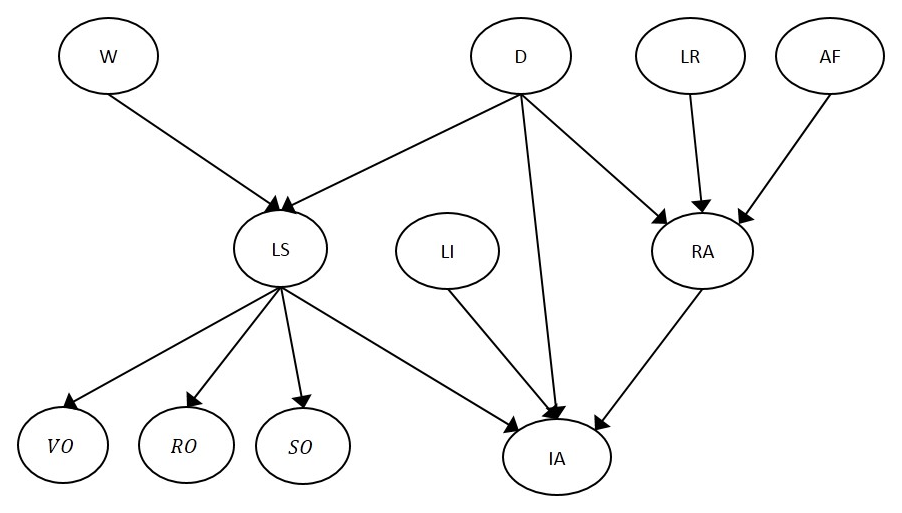
\includegraphics[width=.4\textwidth]{img/causal-model.eps}}
\subfloat[Decision network based on the causal model shown in Figure~\ref{fig:causal-model}\label{fig:decision-graph}]{ \includegraphics[width=.4\textwidth]{img/decision-network.eps}}
 \caption{}
 % decision-graph.eps: 0x0 pixel, 300dpi, 0.00x0.00 cm, bb=-0 -0 424 277
\end{center}
\end{figure*}


\subsection{Bayesian networks}\label{sec:bayesian-networks}

{\red needs to be reworked - Patrick}

A Bayesian network (BN) is a probabilistic graphical model that efficiently represents a joint probability distribution (JPD) over a set of random variables \cite{jensen01book,pearl88book}. A BN is represented through a Directed Acyclic Graph (DAG), where each node in the DAG corresponds to a random variable of the JPD. For example, the causal graph shown in Figure~\ref{fig:causal-model} could describe a DAG of a BN where the scenario variables (solid circles in Figure~\ref{fig:causal-model} are represented as random variables (nodes), and each possible scenario variable state corresponds to a random variable state\footnote{. 
Note that, the range of states for the scenario variables (and therefore the range of states for the random variables) is not determined a priori but as the estimation processes take place, as explained in \cite{conrado14if} on scoping of states.}
For each node given its parents in the DAG, a conditional probability distribution (CPD) needs to be specified. For instance, the CPD $P(LS|D)$ must be specified for the variable $LocationSmuggler$ ($LS$). Discrete CPDs can be represented through conditional probability tables (CPTs).  Since the variables $LS$ and $D$ are discrete, the CPD $P(LS|D)$ can be represented through the CPT shown in Figure~\ref{fig:cpt-example}. This CPT expresses that, given destination X and a small amount of fuel on board, the chance that a refueling action takes place (at location 1) is $0.9$, i.e. $P$($A$~=~Yes~at~1$|$$D$~=~X,~$F$~=~Small) = 0.9. For larger amounts of fuel (and the same destination X), it is estimated that no refueling action takes place. Moreover, there is no chance that the refueling action takes place at locations 2 and 3, as these locations are farther than X itself. This example shows that incompatibility of state combinations can simplify the specification of CPTs for scenario variables, as the probabilities of such combinations are zero.

Before the introduction of BNs, probabilistic inferences were performed directly on a JPD defined over several variables. This, however, limited such operations only to JPDs defined over a small set of variables due to the combinatorial complexity. A Bayesian network, on the other hand, exploits conditional independencies between the random variables. Consequently, the JPD can be factorized into CPDs for each variable in the model. 
For example, considering the BN shown in Figure 5a, the JPD $P(\VV)$ (where $\VV$\footnote{In this section, a single random variable is presented as an uppercase letter and its states as lowercase letters. A set of random variables and of states are shown as bold uppercase and bold lowercase letters, respectively.} = $\{W, D, F, A, I\}$) factorizes into a set of CPDs, i.e.


\begin{eqnarray}
P(\VV) = \prod_i P(X_i|\Pa(X_i)),  \label{eq:chain-rule}
\end{eqnarray}

\noindent
where $\Pa(X_i)$ denotes the parents of node $X_i$. For the BN in Figure 5a, the JPD is therefore

\begin{eqnarray}
 P(W,D,F,A,I) &=& P(W)P(D)P(F)P(A|D,F) \nonumber \\
  & & \cdot P(I|W,D,A). \nonumber
\end{eqnarray}


With the help of the chain rule in Equation~(\ref{eq:chain-rule}), a JPD can be represented through its factorization of CPDs, which requires significant fewer parameters compared to the number of parameters in the JPD. Moreover, by exploiting the conditional independencies between the random variables, efficient exact inference methods can be used, e.g. the junction tree algorithm \cite{cowell99bn}.

The likelihood of scenarios can be computed with the help of Equation~(\ref{eq:chain-rule}), given a BN of the causal model that shows the cause-effect relations between the scenario variables. For instance, for the scenario corresponding to the uppermost complete branch of the scenario tree in Figure~\ref{fig:scenario-tree}, i.e. $W$~=~bad, $D$~=~X, $F$~=~Small, $A$~=~Yes at 1, $I$~=~4, the likelihood can be computed as

\begin{eqnarray}
 P(W=\text{bad}, D=\text{X}, F=\text{Small}, A=\text{Yes at 1}, I=\text{4}) &=& \nonumber \\
 P(W=\text{bad})P(D=\text{X})P(F=\text{Small}) & & \nonumber \\ 
 \cdot P(A=\text{Yes at 1}|D=\text{X},F=\text{Small}) \nonumber \\
 \cdot P(I=\text{4}|W=\text{bad},D=\text{X},A=\text{Yes at 1}). \nonumber
\end{eqnarray}

  
Moreover, one of the main strengths of BNs is the possibility to perform predictive or diagnostic inference based on a given set of evidence denoted by $\E$. For example, in the second phase of the example the weather is observed, i.e. $\E = \{W = \text{bad}\}$. With this observation, the likelihood of the scenarios can be updated by computing $P(\vv|\E)$, where $\vv$ is a configuration of random variables states corresponding to a given scenario. Note that all scenarios with $W = \text{good}$ will get zero probability due to the observation. Assigning zero probabilities to scenarios after an observation update corresponds to pruning of scenarios based on evidence.

Also in the second phase of the example (whose BN is shown in Figure~\ref{fig:bn-example}), a new variable $R$ is added to the model to capture the received refuel report. The model needs to be updated by specifying the CPD $P(R|A)$ as well. The new JPD $P(W,D,F,A,I,R) = P(W)P(D)P(F)P(A|D,F)P(I|W,D,A)P(R|A)$ can be used to re-compute the likelihood of the scenarios, given the occurrence of the refueling report at position 1.




\subsection{Decision Networks}\label{sec:decision-networks}

A {\em decision network (DN)} (also influence diagram or decision graph \cite{russell02bn,howard84rpada,jensen07book}) is a concise graphical and mathematical representation of a decision problem. For example, the BN described in the previous section can be extended into the decision network (DN) shown in Figure~\ref{fig:decision-graph}. This DN consists of the same chance nodes as in the causal model in Figure~\ref{fig:causal-model} plus a decision node $B$ and a utility node $U$. A decision node represents possible actions the decision maker can take. In this case the actions are the different bearings the intercept vehicle can travel, such as North, East, South-west, etc. Next to the decisions we have to model the desirability of the states we end up in after taking an action. This desirability is modeled through the utility node and is dependent on the location of the intercept vehicle and areas. It is desirable that the intercept vehicle is near or at the location of the intercept areas prior to arrival of the smugglers, such that we are able to intercept the smugglers. Thus, the preference of the decision maker can be captured through a utility function that uses the position of the intercept vehicle and intercept areas as arguments.

The location of the intercept vehicle\footnote{In this section we assume there is only a single intercept vehicle} and the smuggler's go-fast constitute a state $s$ in a set of states $\S$ defining the smuggler's domain. However, due to partial observability of the current state, the decision maker (also called agent in decision theoretic literature) has to maintain a belief $P(\S = s | a, \epsilon)$ over the possible states it might be in given an action $a$ and evidence $\epsilon$. The reason for this is that the position of the smugglers is not directly observable after an action $a$, but needs to be estimated from observations $\epsilon$, such as radar, sonar, visual observations or Intel about a possible destination or refueling location (see also causal model in Figure~\ref{fig:causal-model}). Since the agent does not know in which state it is it needs to compute an expected utility based on the utility function $U(s)$ capturing the preferences of the decision maker:

\begin{eqnarray}
 EU(a|\epsilon) = \sum_{s'}P(\S = s'|a, \epsilon)U(s')
\end{eqnarray}

With the help of the expected utility $EU(a|\epsilon)$ the best action $a^*$ can be computed with:

\begin{eqnarray}\label{eq:meu}
 a^* = \argmax_a EU(a|\epsilon)
\end{eqnarray}

Equation~\ref{eq:meu} presents two challenges we need to address in order to compute the best action $a^*$, namely the estimation of $P(\S = s'|a, \epsilon)$ and the computation of the utility using the utility function $U(s')$.


% 
% 
% {\red needs to be reworked - Patrick}
% 
% The BN described in the previous section can be extended into the decision network (DN) shown in Figure~\ref{fig:decision-graph}. This DN consists of the same nodes as in the causal model in Figure~\ref{fig:causal-model} plus a decision node $D$ and a utility node $U$. A decision node represents possible actions the decision maker can take. In this case the actions are the different directions the patrol ship can travel, such as North, East, South-west, etc. The utility node, on the other hand, represents the utility function where the parents of the utility node, i.e. $\{LS,LP,IA\}$, are the arguments of this function:
% 
% \[
%  U(LS,LP,IA) = -\alpha d(LS,LP) - (1-\alpha) d(IA,LP),
% \]
% 
% where $d(X,Y)$ is the distance between $X$ and $Y$ and $\alpha$ is a value between $[0,1]$ that is used to control the importance of either $d(LS,LP)$ or $d(IA,LP)$. In case $\alpha=1$ the utility function is $U(LS,LP,IA) = -d(LS,LP)$ and therefore solely based on the distance between the smuggler's boat and the patrol ship, while $\alpha=0$ the utility function is solely based on the distance of the patrol ship and the intercept area. The choice of $\alpha$ should be based on the information that is available. If more information is available that could help to locate the smuggler's go-fast then we want to weight  $d(LS,LP)$ more by using a higher $\alpha$ value. A higher utility is obtained when the patrol ship is either closer to the smuggler's location or to an intercept area (where eventually the smugglers should travel to).

% In order to evaluate the different decisions modeled in a DN the impact of the decision's consequences need to be measured. The consequence of a decision is measured through a utility node. For example, we need to drive to work either via route A or route B in the shortest amount of time. Clearly in this case the utility is based on the amount of time required to travel to work and the route that results in the lowest amount of time gets a higher associated utility value. In Figure~\ref{fig:decision-graph} an example of a DN is shown with a single decision variable (square node) and utility variable (diamond node) together with several random variables (oval nodes). Since a DN is generalization of a BN we start discussing BNs first.

\begin{figure*}[!t]
\begin{center}
 \includegraphics[width=.95\textwidth]{img/dynamic-decision-graph.eps}
 \caption{Dynamic decision network of the decision network shown in Figure~\ref{fig:decision-graph}.}\label{fig:ddn} 
\end{center}
\end{figure*}


\subsection{Dynamic Decision Networks}

In the Figure~\ref{fig:decision-graph} a decision network was shown for a, so called, one-shot decision. However, intercepting a smuggler that is actively trying to prevent interception governs an environment that is very dynamic. In such environments a one-shot decision is not sufficient and sequential decision making is required to be able to intercept the smugglers. In Figure~\ref{fig:dynamic-decision-graph} a {\em dynamic decision network (DDN)} is shown based on the one-shot DN shown in Figure~\ref{fig:decision-graph}.

\subsection{Partially Observable Markov Decision Process}
{\red connect this to the previous section - Tom \& Patrick}

A Markov Decision Process (MDP) \cite{bellman1957dynamic,mdp} describes synchronous interactions between an agent and the world. MDPs are used to model sequential decision making problems. At each time-step an agent takes an action that changes the state of the world. The agent can collect rewards, which are received when it takes certain actions in certain states. An MDP is formally described as the tuple $\langle\S,\mathcal{A},T,R,\gamma\rangle$:

\begin{itemize}
\item $\S$ is the set of states of the world,
\item $\mathcal{A}$ is the set of actions,
\item $T:\S\times\mathcal{A}\to\P(s'|a,s)$ is the state transition function \ie the probability of moving to state $s'$ given that action $a$ was performed in state $s$,
\item $R:\S\times\mathcal{A}\to\mathbb{R}$ is the reward function, which maps each state-action pair to a real reward. Note that this can represent a cost, \ie $r < 0$,
\item $\gamma$ is the discount factor, representing the difference in preference between present and future rewards.
\end{itemize}

The state space $\S$ of an MDP can be factored, meaning that it is represented by a discrete set of state variables. As such, the state $\S$ can be described as a vector $\left(X_1,\ldots,\X_n\right)$ where each variable $X_i$ can take on a value in its domain. 

The goal of an MDP is to find a policy $\pi:\S\rightarrow\mathcal{A}$ that maps states to actions such that the reward is maximized. Often, a horizon $h$ is introduced to limit the look-ahead distance. In the case of MDPs the assumption is made that an agent can fully observe the world, as is the case in for instance games of complete information like Chess or Checkers. However, in many real-world domains, the state of the world is not fully observable, and the agent cannot determine the state it is in with complete accuracy. To represent this uncertainty over the agent's current state and observations, the MDP model can be extended to the Partially Observable MDP (POMDP) \cite{aastrom1965optimal,pomdp}. A POMDP can be formally described as $\langle\S,\mathcal{A},T,R,\Omega,O,\gamma\rangle$:

\begin{itemize}
\item $\S,\mathcal{A},T,R,$ and $\gamma$ describe the Markov Decision Process,
\item $\Omega$ is the set of possible observations,
\item $O:\S\times\mathcal{A}\to\P(o|a,s')$ is the probability of observing $o$ in state $s'$, after performing action $a$. 
\end{itemize}

POMDP's require an agent to maintain an internal {\it belief state}, in which all knowledge about the current state is summarized. POMDP's are harder to solve exactly than MDP's, and require approximate methods to be used in real-world problems \cite{pineau2006anytime}.

The MDP approach has been extended to include multi-agent decision-making, \ie MMDP and MPOMDP. In these cases, the action space $\mathcal{A}$ represents the joint-actions $\A_{m} = \A_1\times\ldots\times\A_n$ of all $n$ agents under consideration. Where solving an MDP can be performed in polynomial time, solving multi-agent problems suffer from the fact that their action space increases exponentially with the number of agents.

In Section \ref{sec:scenario-based-dm} we will use the POMDP model developed in this section to detail an approach to planning and decision-making under uncertainty in the smuggler use-case.

% Making decisions based on a POMDP defined in the previous section

\section{Scenario-Based Decision-Making}
\label{sec:scenario-based-dm}

{\red explain what we want to do, why do we need to plan, what is the role of scenarios, what kind of decisions do we want to make? assumptions made! - Tom \& Patrick}

\subsection{Planning Under Uncertainty}

{\red Method to find decisions based on repeated sampling of the state-space. requires: Discrete action model and state space, and a method of defining the current belief of the smuggler's location. - Tom}

\subsection{State Representation}
\label{sub:staterep}

The state represents the locations of the set of agents $\Psi$ under consideration for the planner. Each agent $\psi_i$ occupies a single location on a geographical map. Where the map is defined by the underlying geographical area in which the scenario is located.

The maritime security domain generally plays out over a sizable area. Based on the problem, the area of interest can span over  dozens of kilometers. Planning on a (near-)continuous state space would soon become intractable based on the number of hidden locations for the smuggler and action spaces for the intercept vehicles. Therefore we propose a framework in which an area of interest is factored into discrete elements before or at the start of an operation. Based on the surface-area of interest and the required precision of the mission, a location of interest is selected on a geographical system, which is then divided into discrete cells.

Given the factored state space $S = \left(X_1,\ldots,X_n\right)$, the domain of each variable $X_i$ can be defined by the occupying agent(s) \ie $x_i=\left(x_{i1},\ldots,x_{ik}\right)$, where $x_{ij}\in\Psi$. Each variable's domain is restricted based on the underlying geographic characteristics \ie boats can only occupy a location on water. Moreover, political borders and no-fly zones can further restrict the domain of each variable.

{\red How do we represent the possible states - Tom}

\subsection{Belief State Estimation with Context}

In the defined state representation, the locations of the friendly {\red define friendly/hostile somewhere, perhaps bluefor and opfor are better terms?} agents are assumed to be known at each point in time. This assumption is based on the availability of GPS localization and wireless communication techniques. However, the location of the smuggler is unknown to the agents and therefore our planner. Given that the goal of the multi-agent plan is to locate, track and capture the smuggler, respectively, the combined set of agents needs to maintain a belief over the current location of the smuggler's go-fast.

{\red also explain that we do not know the exact location of the go-fast, and that we expect only sparse and/or unreliable observations}
{\red how do we estimate the position of the smugglers based on the observations and the context: description of particle filter - Rik}

\subsection{Multi-Agent Decision-Making}

{\red some thoughts on how to handle these kind of problems (i.e. MPOMDP or DEC-POMDP, using MCTS (UCT/BRUE etc)) - Tom \& Patrick}
% Cite Ad hoc Autonomous agent teams
% Cite multi-agent II pursuit games

\section{Conclusion}
\begin{itemize}
\item Summarize what we discussed in the paper
\item State what the next steps are
\item Future work
\end{itemize}

\section*{Acknowledgment}

\bibliographystyle{IEEEtran}
\bibliography{tombib,BNbib}

% that's all folks
\end{document}